\documentclass{article}

\usepackage{amsmath,graphicx}
\usepackage{sectsty}
\usepackage[letterpaper, margin=1.75cm, top=1.75cm]{geometry}
\usepackage{amsmath,graphicx}
\usepackage{multicol}
\usepackage{array}
\usepackage{csvsimple}
\usepackage{booktabs}
\usepackage{multirow}
\usepackage{float}
\usepackage{array}
\usepackage[font=small,labelfont=bf]{caption}
\usepackage{booktabs}
\usepackage{algorithm}
\usepackage{algorithmic}
\usepackage{csvsimple}
\usepackage{biblatex}

\addbibresource{refs.bib}

\newenvironment{Figure}
    {\par\medskip\noindent\minipage{\linewidth}}
    {\endminipage\par\medskip}

\newcommand{\centered}[1]{\begin{tabular}{l} #1 \end{tabular}}

\def\code#1{\texttt{#1}}
\def\bigO#1{$O(#1)$}

\makeatletter
\def\BState{\State\hskip-\ALG@thistlm}
\makeatother

\title{Simulated Annealing}
\author{
    Anderson, Colin
    \and
    Bess, Brady
    \and
    Kartchner, Shaylee}
\date{}

\begin{document}

\maketitle

\noindent\makebox[\linewidth]{\rule{\textwidth}{0.4pt}}

\begin{center}
    \textbf{Abstract}
\end{center}

The Traveling Salesperson Problem (TSP) is a highly studied and well-known problem in computational complexity theory and computer science.  It asks the question “what is the shortest path through a group of cities where each city will be visited once before returning to the original city?” Although it is an NP-hard problem, many algorithms and solution patterns have been created to solve the TSP.  This report describes two of these algorithms, a greedy algorithm and simulated annealing, and analyzes their effectiveness in finding an optimal and computationally efficient solution.  Through implementation and testing of the algorithms against a variety of problem sizes, it was discovered that a simulated annealing approach can reduce the optimal path found by a greedy implementation by 10-13\%.  This path optimization comes with runtime cost, however, as the randomness of neighbor-finding in our simulated annealing algorithm makes it costly.  

\noindent\makebox[\linewidth]{\rule{\textwidth}{0.4pt}}

\begin{multicols}{2}
    \section{Introduction}

    This report will showcase two algorithms for solving TSP problems. First a greedy approach will be introduced and discussed.  In general, greedy algorithms can be applied to different optimization problems involving multiple steps or iterations, and characteristically they seek solutions by choosing the most appealing local value during each iteration, neglecting to look ahead, which could allow for increased optimization.  The strategy and the time complexity of a greedy implementation will be explained.
    
	Afterwards, a simulated annealing approach will be introduced.  With the metallurgical heat treating and cooling process of annealing as its computational model, simulated annealing demonstrates a search that becomes more refined and favorable as our problem set is “cooled” over time.  Probability and a simulated “temperature” factor into the locality explored in the global search space, and during high temperature iterations there is a greater chance of switching localities by choosing a less optimal neighboring path.  This is done in hopes of escaping local optimizations that may appear to the algorithm as global optimizations.  An explanation of the time complexity of simulated annealing as well as an analysis of empirical study of simulated annealing to solve TSP problems will be presented.

    \section{Greedy Algorithm}
    \subsection{Description}

    The greedy approach to the TSP begins at each city and chooses to visit the next closest unvisited city.  It will continue to visit closest unvisited cities until all cities have been visited, where it will then return to the city where it began.  In this approach long travels to far away cities are meant to be eliminated, assuring our cost stays as low as possible.  

    Running the greedy approach once for every city as a starting point gives a great baseline minimum tour, and in cases where the city-tree structure is a fully connected (complete) graph, is a sort of exhaustive brute force way to find the optimal tour with high probability.  However in many problem cases it is not guaranteed every city will be connected to every other city.  In these cases the algorithm will hit a dead end in its greedy search and return an invalid path, making finding optimal path length in these situations highly unlikely.  Still, the greedy algorithm will return better results than a randomly created tour.   

    \subsection{Complexity Analysis}
    \subsubsection{Time}
    This approach takes \bigO{n^3} time. The algorithm starts with a city, and picks the next shortest path. To find the shortest path, it has to loop through every available path, which is \bigO{n}. It has to do this at every step, so that gives us \bigO{n^2}. This could potentially find a valid solution, but there is no guarantee it will find a valid path with the initial starting city, or that the path it finds will be the best greedy solution. Because of this, we chose to run the algorithm starting with every city, ensuring we find the best possible greedy solution. This means the algorithm repeats the \bigO{n^2} process with every city, so we end up with \bigO{n^3} time complexity.
    
    \subsubsection{Space}

    The space complexity, however, only costs \bigO{n^2}. To calculate the best path, a two-dimensional cost matrix is created, which costs \bigO{n^2} space. Each route takes up \bigO{n} space, which is written over with each iteration, saving only the best path.

    \section{Simulated Annealing}
    \subsection{Description}

        Simulated Annealing is an approach to finding and optimal solution without getting stuck in a local minima. The basic concept is that you find a random solution. Then find a random neighbor to that solution. If that neighbor is a better solution, then keep it. If it isn’t, then there is a chance that you will take it anyways because it might lead to a better solution. 

        This makes more sense when looked at in the context of annealing. Annealing is a heat treatment applied to metal in order to reduce hardness and increase flexibility. Flaws in the metal make it rigid, but when you heat metal up these flaws can shift and move through the metal. As it cools these flaws are locked in place. The principle that carries over to simulated annealing is that the flaws can move freely at high temperatures, but as the metal cools it becomes increasingly hard for them to move.
        
        The pseudo-code for a generic simulated annealing algorithm is as follows (\,this pseudo-code comes from wikipedia \cite{wikiAnn})\,:

        \begin{Figure}
            \captionof{figure}{Simulated Annealing Pseudocode}\label{anneal}

                \begin{algorithmic}[1]
                \STATE $\textit{s} \gets s_0$
                \FOR{$k=0$ through $k_{max}$}
                \STATE $T \gets \text{temperature}((k+1)/k_{max}))$
                \STATE $s_{new} \gets $randomNeighbor$(s)$
                \IF {$\textit{cost}(s_n) \le \textit{cost}(s)$}
                \STATE $s \gets s_n$.
                %\Else\ \textbf{if} $P(\textit{cost}(s),\textit{cost}(s_n), T) \ge \text{random}(0,1)$\ \textbf{then}
                \ELSIF{$P(\textit{cost}(s),\textit{cost}(s_n), T) \ge \text{random}(0,1)$}
                \STATE $s \gets s_n$.
                \ENDIF
                \ENDFOR
                \RETURN s
            \end{algorithmic}

        \end{Figure}

        The procedure begins with selecting an initial solution $s_0$ and storing it as $s$. Then a temperature $T$ is found. The value of $T$ starts high and reaches 1 as $k \rightarrow k_{max}$. Then a random ``neighbor'' of $s$ is selected, this is $s_n$. The cost of $s_n$ is compared to the cost of $s$. If $s_n$ is cheaper, then it replaces $s$. However, if it is not, then the cost of each solution, as well as the temperature, are passed into a probability function \code{P()}. When $T$ is large, there is a high chance that \code{P} will return a number that is larger than \code{random(0,1)}. This means that at high temperatures (small values of $k$) the algorithm will likely select solutions that are more expensive than the previous one. This allows the algorithm to ``jump'' out of local minima.

        \begin{center}
            \begin{minipage}{0.9\columnwidth}
                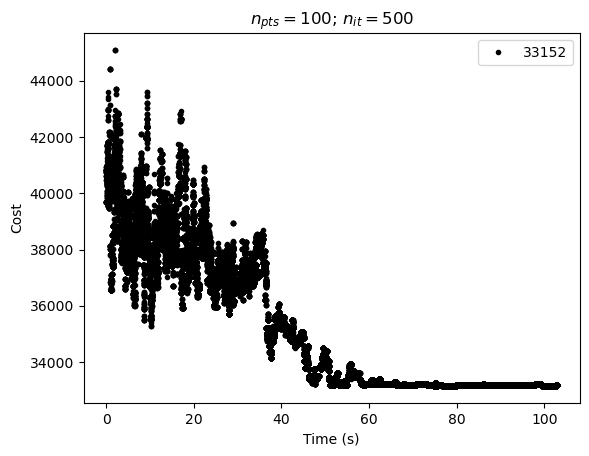
\includegraphics[width=\columnwidth]{./sVal100/Annealing_100Pts_500it.png}
                \captionof{figure}{Example solution pattern}\label{exam}
            \end{minipage}
        \end{center}
        
        Figure \ref{exam} shows an example of the algorithm converging to a solution. Early in the algorithm, the cost of the selected solution often increases, but as the temperature decreases the algorithm selects more expensive solutions less and less. Eventually $T$ reaches 1 and the algorithm returns the selected solution.

        When implementing a simulated annealing algorithm there are a few design questions that have a large impact on the algorithm's effectiveness. First, you need to figure out what defines a given solution's ``neighborhood''. The ``neighborhood'' consists of other solutions that are similar to the current solution. 
        
        Research indicated that a common approach to finding a neighbor for the TSP just involves randomly selecting a continuous group of cities and reconnecting them randomly \cite{tspWeb}. This is a very effective method for fully connected graphs, but our graph has missing edges, so placing the cities in a random order at large problem sizes very rarely yielded a valid path. 
        
        We overcame this issue by using our greedy algorithm to connect the cities that we pulled out. We took the first city removed and set the shortest path out of it to infinity. If we didn't do that we would end up with the exact same order as before. If removing that edge made the problem unsolvable, we just tried again with the second city removed, and so on.
        
        Once the neighborhood has been defined the following items also need to be developed:

        \begin{itemize}
            \item {Annealing schedule}
            \item {Number of Iterations}
            \item {Starting temperature}
            \item {Probability Function}
        \end{itemize}

        To answer these questions we did some research and found a website which implemented an annealing algorithm to solve a TSP problem (written in R and used on fully connected TSP problems) \cite{tspWeb}. We used that code base as our source of many equations and relationships at the heart of our code. 

        The annealing schedule refers to the \code{temperature} function on line 2 of Figure \ref{anneal}. This function dictates the cooling curve for the algorithm. An aggressive function, such as exponential decay, can cause the algorithm to freeze up early and converge to a local solution. A sluggish function, such as linear decay, and cause the algorithm to keep ``bouncing'' out of solutions all the way to it's completion. A function that balances the two should be used. We used the following function for our annealing schedule:

        \begin{equation}
            T = \frac{2T_{max}}{1 + \exp{(x/100)}}
        \end{equation}

        This equation came from the source code we obtained from Todd Schneider's website \cite{tspWeb}.

        The number of iterations doesn't affect the difference between $T_{max}$ and $T_{min}$, but it does dictate how quickly a solution is reached. More iterations will slow the algorithm down and give it time to move towards the optimal solution. We decided to make the number of iterations dependent on the problem size.

        \begin{equation}
            k_{max} = 100\cdot n_{cities}
        \end{equation}

        We decided on this relationship after experimenting with the iteration count. Further discussion on this can be found in Section \ref{results}.

        The starting temperature $T_{max}$ impacts how easy it is for the algorithm to move from a solution to a less-optimal neighbor. Section \ref{results} will contain more of our analysis of this. As we did with $k_{max}$, we made the starting temperature dependent on the problem size. The justification behind this was that larger problems require the algorithm to ``jump around'' more to try and find the optimal solution. The following equation related the problem size to $T_{max}$:

        \begin{equation}
            T_{max} = 5\cdot k_{max}
        \end{equation}

        The probability function refers to \code{P()} on line 7 of Figure \ref{anneal}. This function relates the difference in cost between $s$ and $s_n$ with the current temperature to randomly determine if the algorithm will move to $s_n$ or not. This has a similar impact on the algorithm as the annealing schedule. If it is easy to move to neighbors then it is easier to move towards the optimal solution. But if it is too easy then the algorithm can move past the optimal solution and settle on a local minima as it cools. We decided on the following probability function (\,again from Todd Schnieder's website \cite{tspWeb})\,:

        \begin{equation}
            \exp{\Big(\frac{-(s_n - s)}{T}\Big)} \ge \text{random}(0,1)
        \end{equation}

        \subsection{Complexity Analysis}
        \subsubsection{Time}

        The time complexity for our simulated annealing approach is \bigO{n^3}. The algorithm first generates a valid path by using the greedy approach described above, which was determined to cost \bigO{n^3}. This initialization is only run once. After this, the algorithm finds a neighbor to the initial path. This involves randomly picking two indices in the initial path, and greedily finding a new way between the two. This process is only repeated once; even if a valid path is not found, the algorithm simply continues and generates a new neighbor. This means that generating the neighbor only costs \bigO{n^2}, since we omit the step in the initial greedy approach of checking every starting node. 
        
        After this, the algorithm compares the costs between the initial path and the cost of the newly generated neighbor. If the new path is shorter, it is chosen to continue to the next iteration. If not, it may randomly be chosen in the simulated annealing process. All of this comparison costs \bigO{n}. 
        
        This process of generating a new neighbor and comparing the two path costs is repeated $n * p$, where $p$ is the number of iterations per city. Ultimately, we decided to make $p$ a constant, so the process is repeated \bigO{n} times. This gives us a total time complexity of \bigO{n^3}.
    
        \subsubsection{Space}

        In terms of space complexity, the function that generates a new neighbor creates a cost matrix to determine valid paths, which gives the function a space complexity of \bigO{n^2}. The only other space needed in the algorithm is that of the current path and neighbor path, which each cost \bigO{n}. Overall, then, the space complexity for this simulated annealing algorithm is \bigO{n^2}.
        
        \section{Results and Analysis}\label{results}
        \subsection{Empirical Results}

        The first results that we have are related to the number of iterations in a given solution. We were unsure how many iterations to do, so we ran our algorithm at various iteration counts. The results of our experiments can be found in Table \ref{iterGraph}. It is worth noting that the number of iterations referenced on the table is multiplied by the problem size (\,number of cities)\, to get the actual number of iterations for each run.
        
    \end{multicols}

    \begin{minipage}{0.8\paperwidth}
        \captionof{table}{Tour Distance Over Time at Various Iteration Counts}\label{iterGraph}
        \begin{tabular}{cccccc}
            \toprule
            \multicolumn{1}{c|}{
                \parbox[t]{1.5cm}{\begin{small}Number\\ of cities\end{small}}} & 
            \multicolumn{5}{c}{Number of Iterations} \\
            \midrule
            
            & 50 & 100 & 250 & 500 & 1000 \\
            
            15 &
            \centered{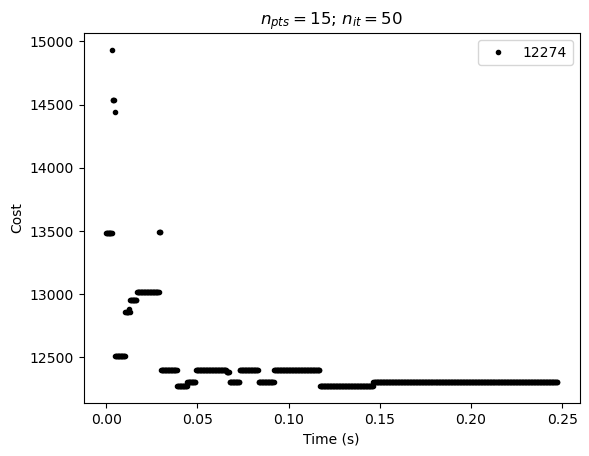
\includegraphics[width=0.126\textwidth]{sVal100/Annealing_15Pts_50it.png}} &
            \centered{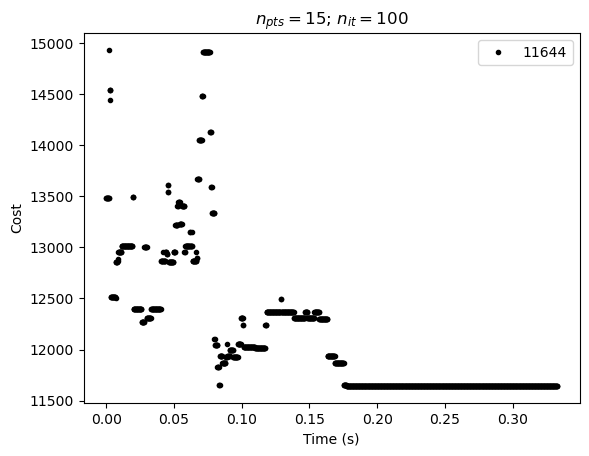
\includegraphics[width=0.126\textwidth]{sVal100/Annealing_15Pts_100it.png}} &
            \centered{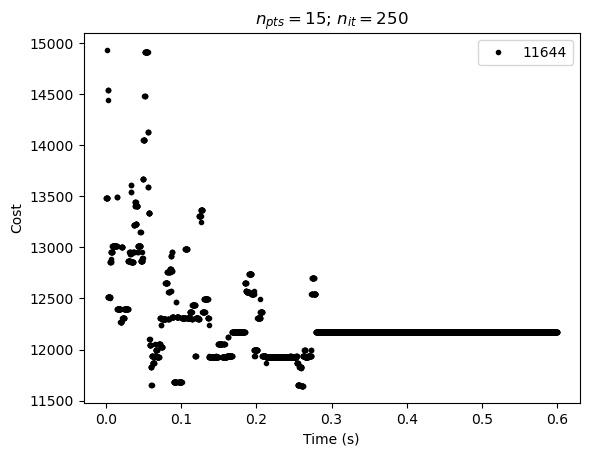
\includegraphics[width=0.126\textwidth]{sVal100/Annealing_15Pts_250it.png}} &
            \centered{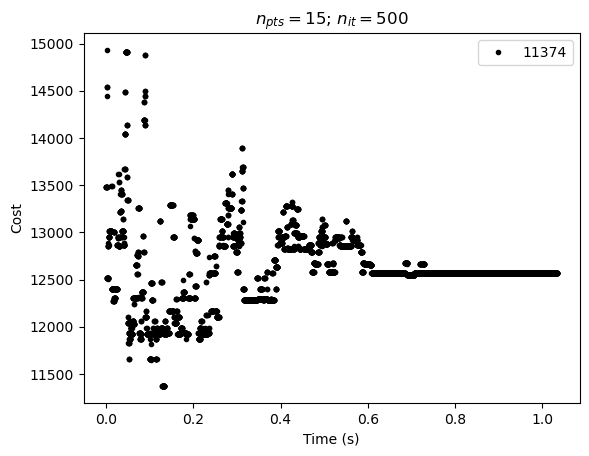
\includegraphics[width=0.126\textwidth]{sVal100/Annealing_15Pts_500it.png}} &
            \centered{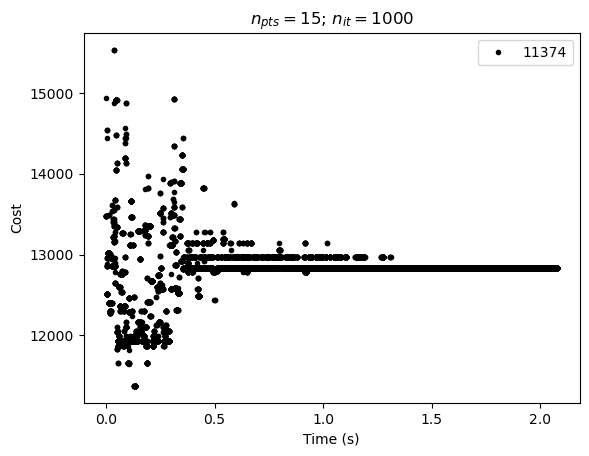
\includegraphics[width=0.126\textwidth]{sVal100/Annealing_15Pts_1000it.png}} \\
            
            30 &
            \centered{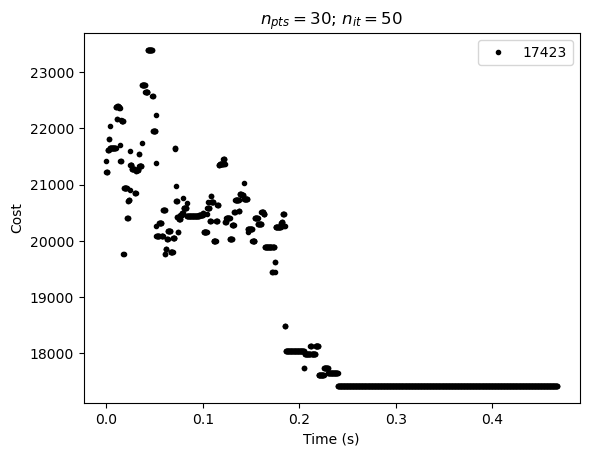
\includegraphics[width=0.126\textwidth]{sVal100/Annealing_30Pts_50it.png}} &
            \centered{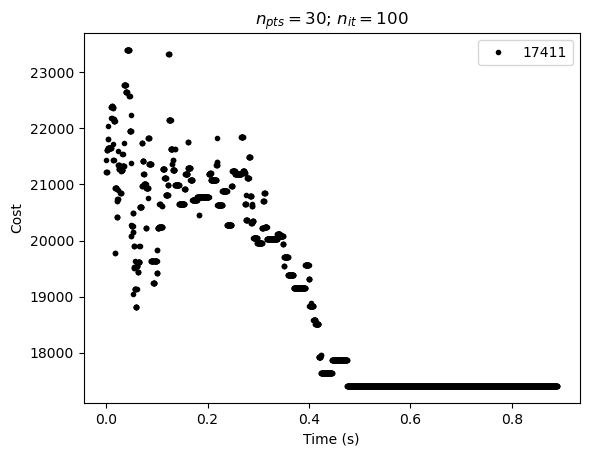
\includegraphics[width=0.126\textwidth]{sVal100/Annealing_30Pts_100it.png}} & 
            \centered{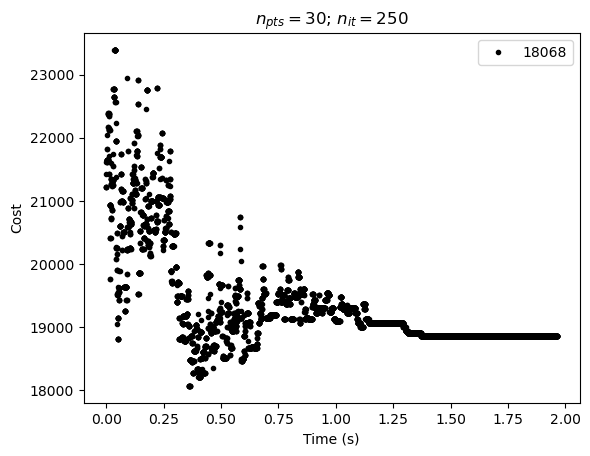
\includegraphics[width=0.126\textwidth]{sVal100/Annealing_30Pts_250it.png}} & 
            \centered{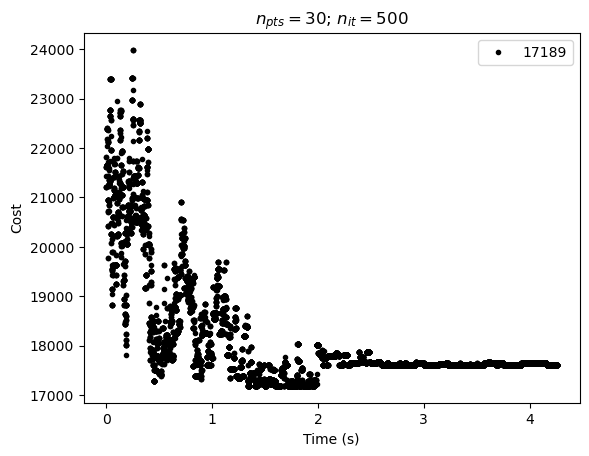
\includegraphics[width=0.126\textwidth]{sVal100/Annealing_30Pts_500it.png}} & 
            \centered{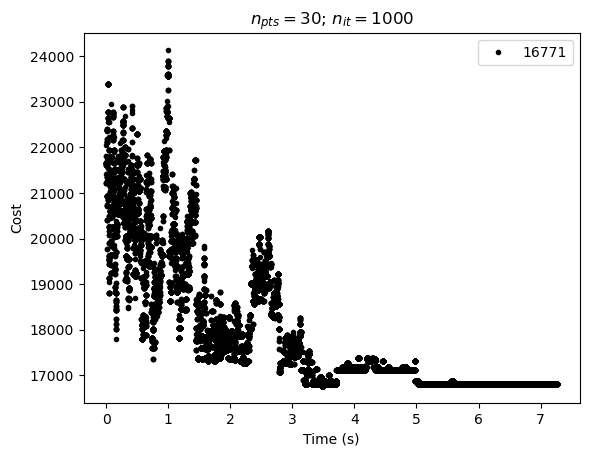
\includegraphics[width=0.126\textwidth]{sVal100/Annealing_30Pts_1000it.png}} \\
            60 &
            \centered{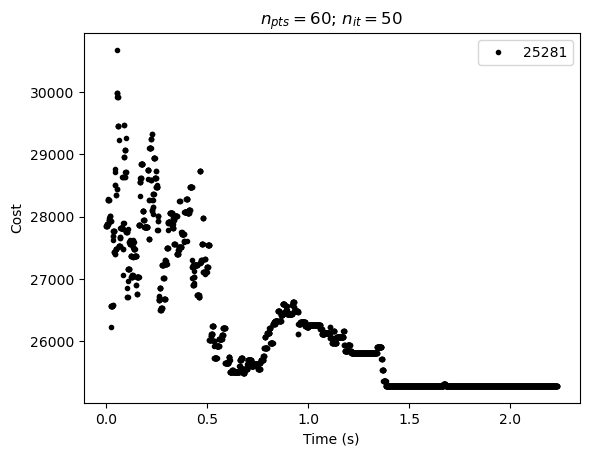
\includegraphics[width=0.126\textwidth]{sVal100/Annealing_60Pts_50it.png}} &
            \centered{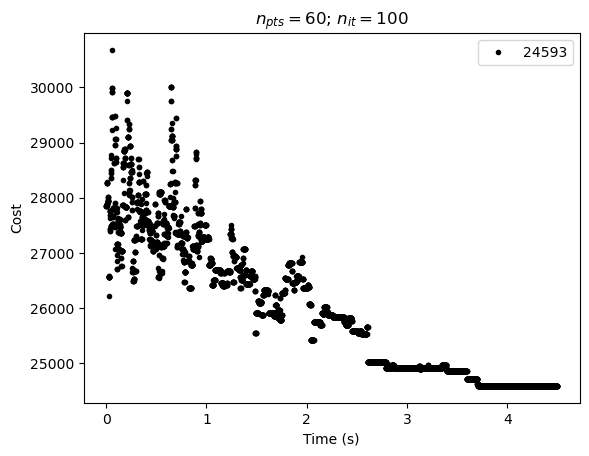
\includegraphics[width=0.126\textwidth]{sVal100/Annealing_60Pts_100it.png}} &
            \centered{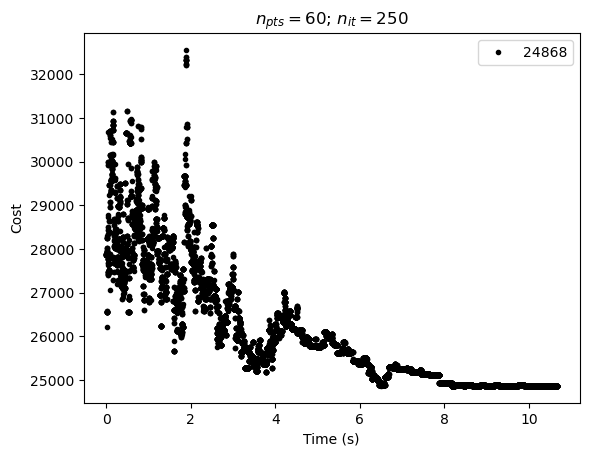
\includegraphics[width=0.126\textwidth]{sVal100/Annealing_60Pts_250it.png}} & 
            \centered{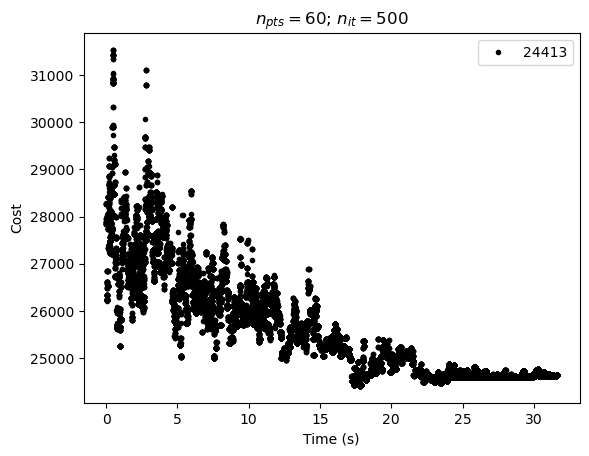
\includegraphics[width=0.126\textwidth]{sVal100/Annealing_60Pts_500it.png}} &
            \centered{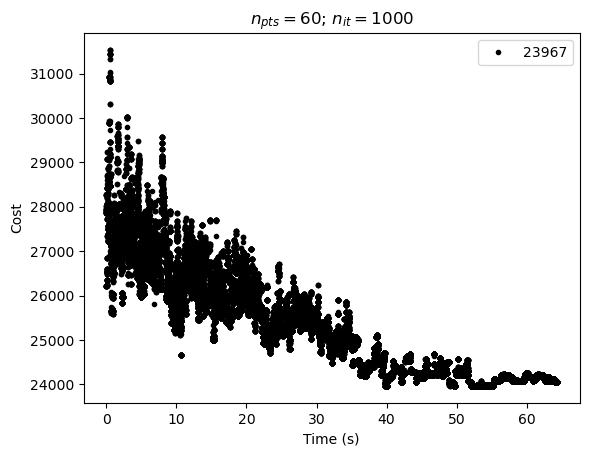
\includegraphics[width=0.126\textwidth]{sVal100/Annealing_60Pts_1000it.png}} \\
            100 &
            \centered{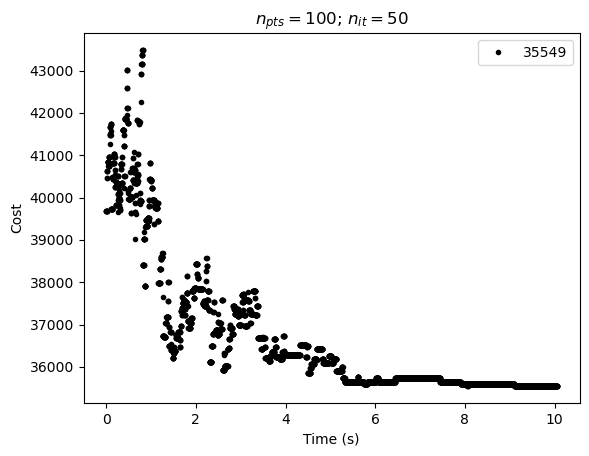
\includegraphics[width=0.126\textwidth]{sVal100/Annealing_100Pts_50it.png}} &
            \centered{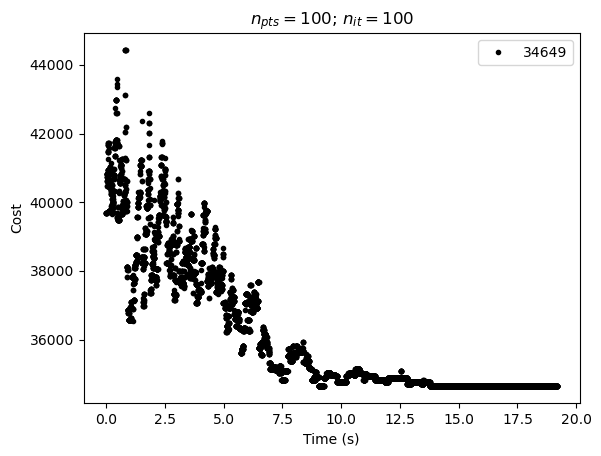
\includegraphics[width=0.126\textwidth]{sVal100/Annealing_100Pts_100it.png}} &
            \centered{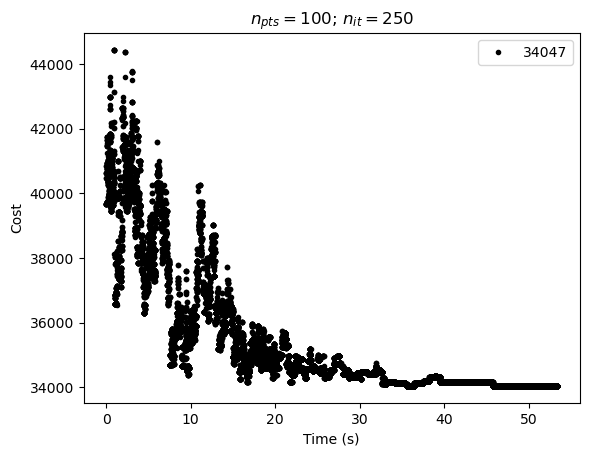
\includegraphics[width=0.126\textwidth]{sVal100/Annealing_100Pts_250it.png}} &
            \centered{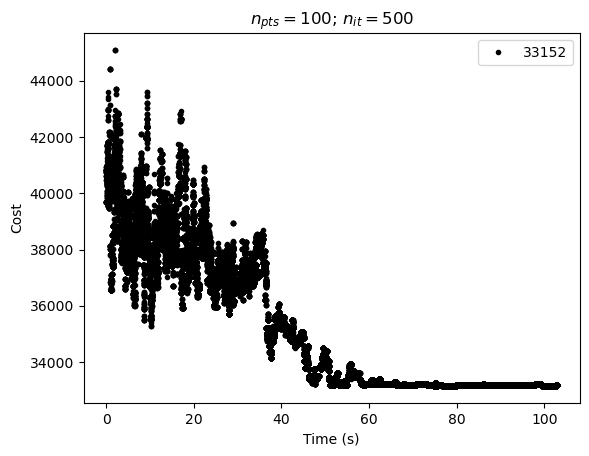
\includegraphics[width=0.126\textwidth]{sVal100/Annealing_100Pts_500it.png}} &
            \centered{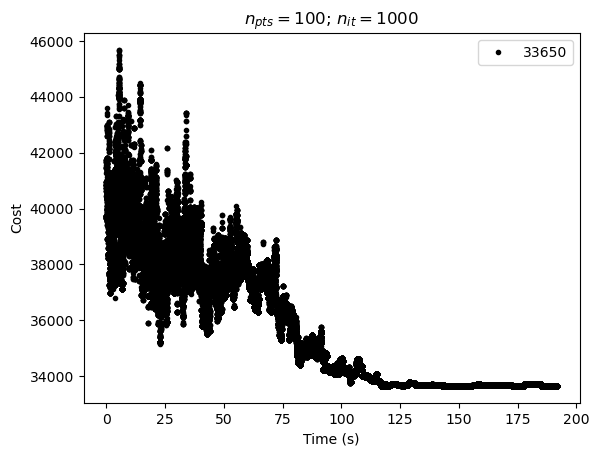
\includegraphics[width=0.126\textwidth]{sVal100/Annealing_100Pts_1000it.png}} \\
            200 &
            \centered{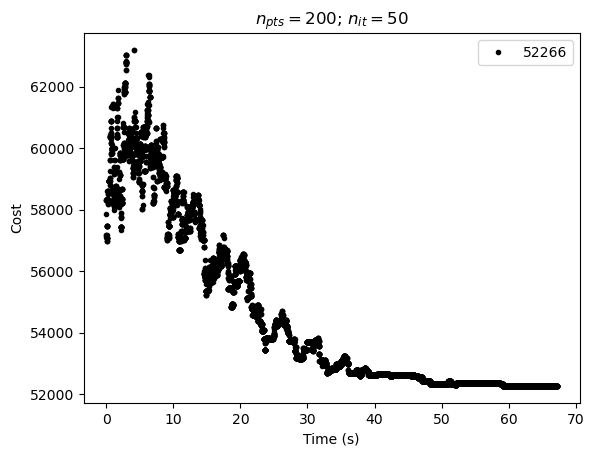
\includegraphics[width=0.126\textwidth]{sVal100/Annealing_200Pts_50it.png}} &
            \centered{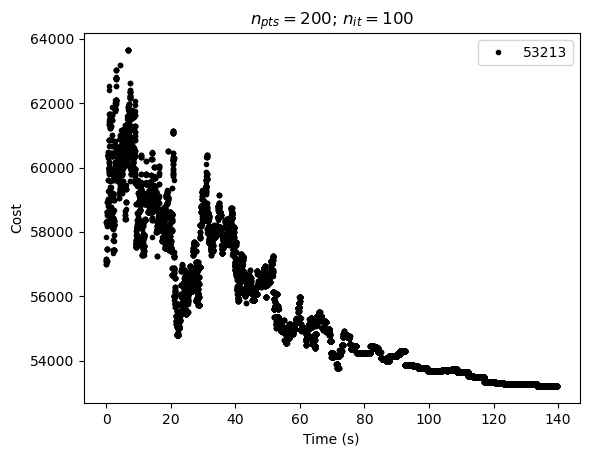
\includegraphics[width=0.126\textwidth]{sVal100/Annealing_200Pts_100it.png}} &
            \centered{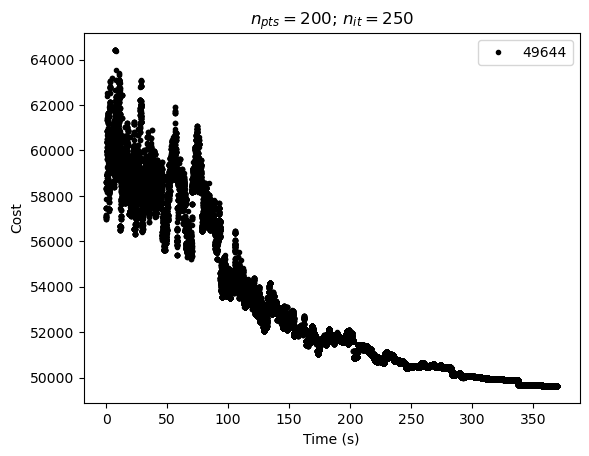
\includegraphics[width=0.126\textwidth]{sVal100/Annealing_200Pts_250it.png}} & 
            \centered{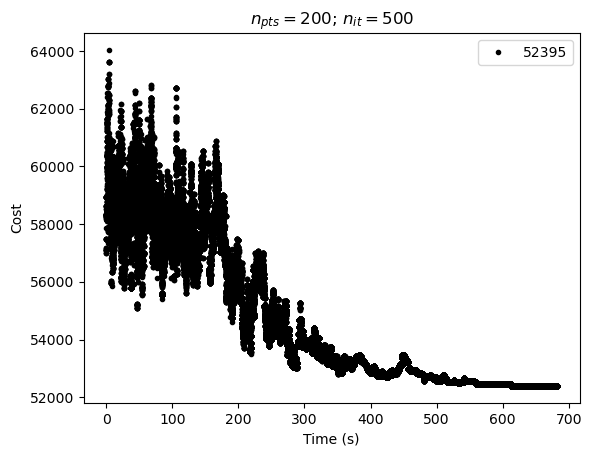
\includegraphics[width=0.126\textwidth]{sVal100/Annealing_200Pts_500it.png}} & 
            \centered{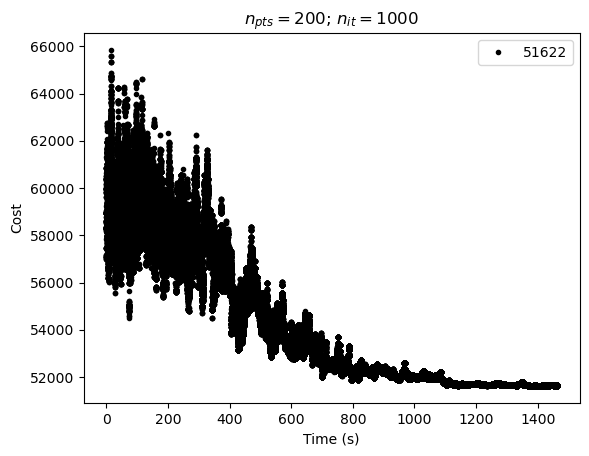
\includegraphics[width=0.126\textwidth]{sVal100/Annealing_200Pts_1000it.png}} \\
        \end{tabular}
    \end{minipage}
    
    
        In analyzing the final solution value for each of the runs in Figure \ref{iterGraph} we found that the run with the greatest number of iterations didn't always yield the best solution. Because of this, we decided to favor runtime and decrease the number of iterations to 100 per city. 

        After determining that increasing the number of iterations didn't guarantee a better solution we began to look at the starting temperature (\,$T_{max}$)\,. However, we ran out of time to do a thorough analysis of this. A future project could be doing thorough testing of the impact the number of iterations and $T_{max}$ have on the final solution. A correlation could even be developed to dynamically choose $T_{max}$ and the number of iterations based on problem size.

        Once we decided on doing 100 iterations per city we were able to do our time trials of our algorithm. The results of these experiments are found in Table \ref{expRes}
    

        \begin{minipage}{0.8\paperwidth}
            \begin{center}
            \captionof{table}{Experimental Data}\label{expRes}
            \scalebox{0.65}{
                \csvreader[
                respect all,
                autotabular
            ]{data.csv}{}{\csvlinetotablerow}
            }
            \end{center}
        \end{minipage}

    \begin{multicols}{2}
        The branch and bound algorithm consistently out performed our annealing algorithm in terms of cost of tour. However, the branch and bound algorithm at 100 cities and above always timed out at 10 minutes, while our annealing algorithm only timed out when doing 200 cities with 500 or more iterations per city. For example, at 100 cities the branch and bound algorithm timed out while our annealing algorithm only took 20 seconds. The final entry in our table was done out of curiosity. Doing 200,000 iterations over 200 cities took 24 minutes and only resulted in an improvement to the cost of about 1\%.

        In running timers in our code we saw that it was our neighbor finding algorithm that took almost all of the runtime. As stated previously, we just used a greedy algorithm to find a neighbor by swapping the order of the cities. This is a case where we have an efficient algorithm because we push the complexity into a different problem. That is another source of future work; research into fast path-finding algorithms. It should be interesting because we don't care about the cost of the path, we just want to find a valid path fast.

        Looking at how our algorithm performed at different iterations per city we see that our earlier assumption that increasing the iterations did not guarantee a better solution was correct. Obviously the iterations per city is only one factor and we would need to do additional testing to determine the best combination of parameters that would optimize our algorithm.
    \end{multicols}

\pagebreak
\subsection{Screenshots}

    \begin{minipage}{0.8\paperwidth}
        \captionof{table}{Typical Results}\label{screen}
        \begin{tabular}{cc}
            \toprule
            Greedy & Annealing \\
            \midrule
            \centered{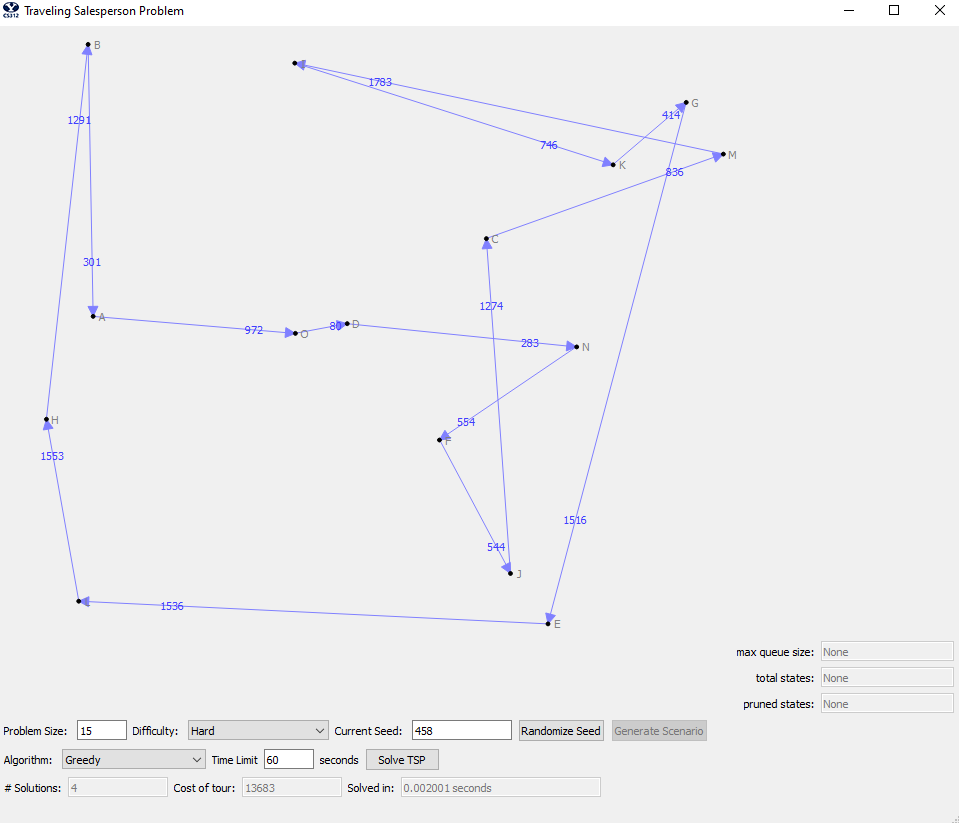
\includegraphics[width=0.35\paperwidth]{sVal100/15_Greedy.png}} &
            \centered{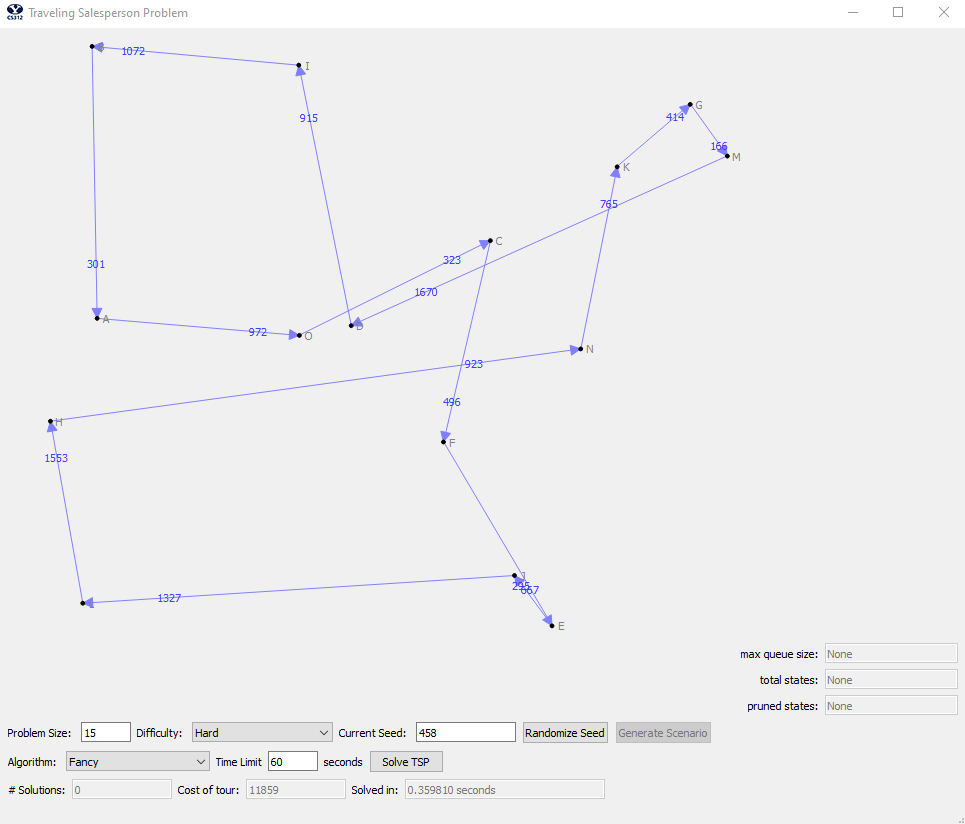
\includegraphics[width=0.35\paperwidth]{sVal100/15_Fancy.png}} \\
            \centered{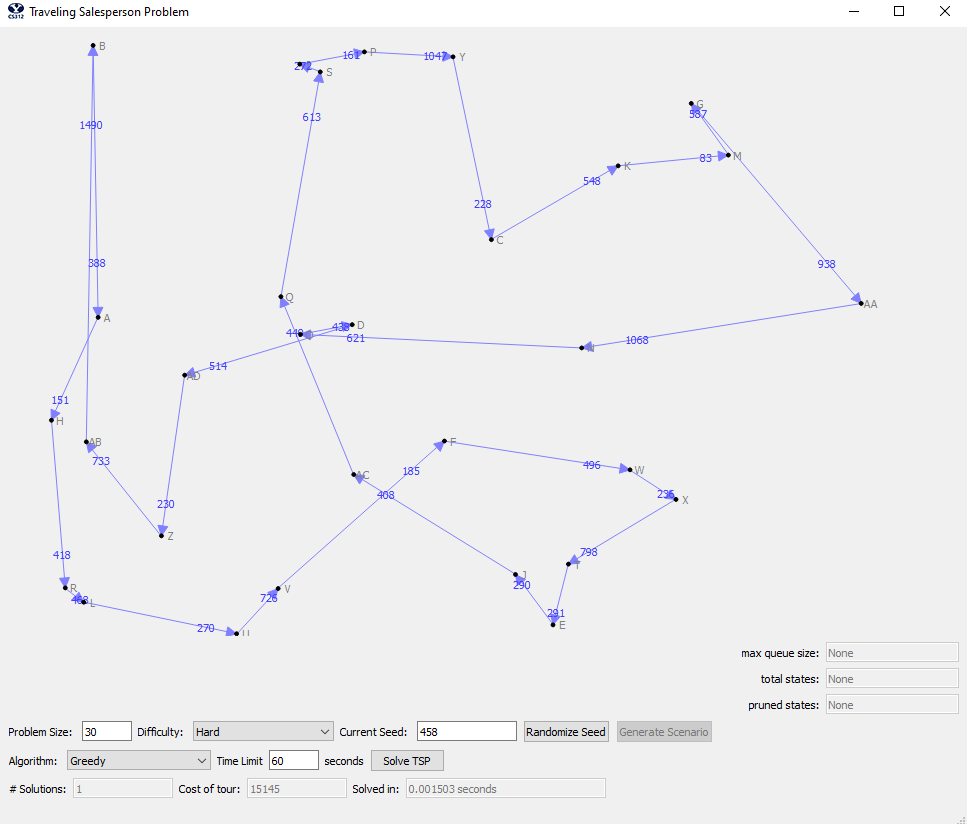
\includegraphics[width=0.35\paperwidth]{sVal100/30_Greedy.png}} &
            \centered{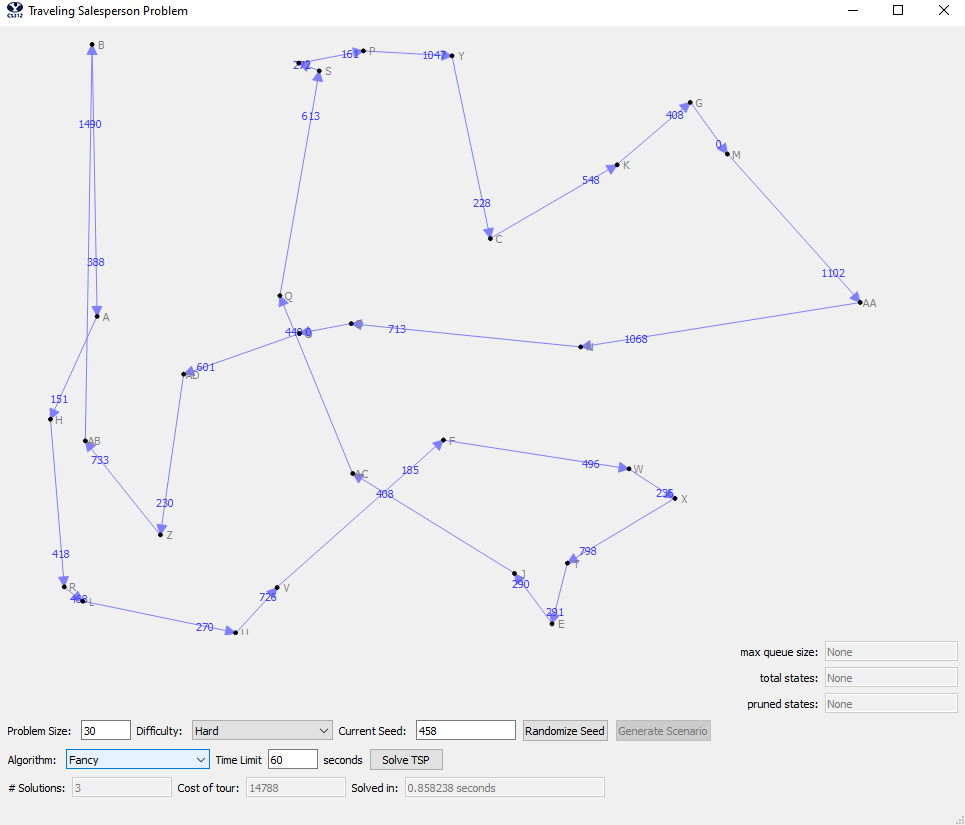
\includegraphics[width=0.35\paperwidth]{sVal100/30_Fancy.png}} \\
            \centered{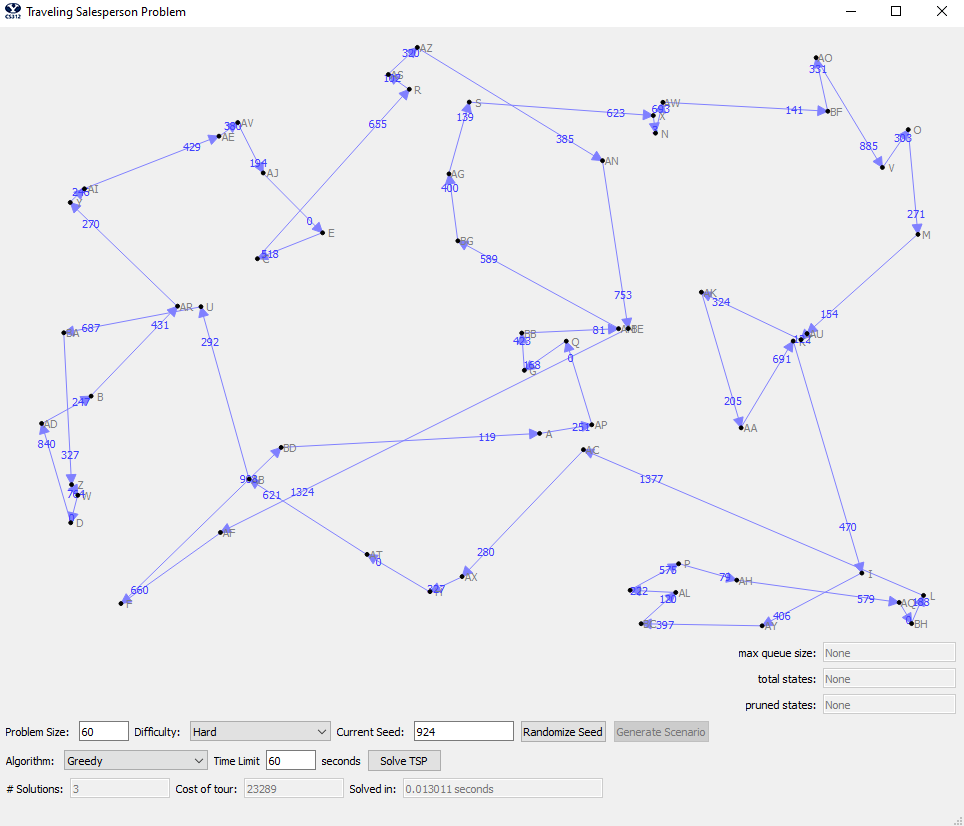
\includegraphics[width=0.35\paperwidth]{sVal100/60_Greedy.png}} &
            \centered{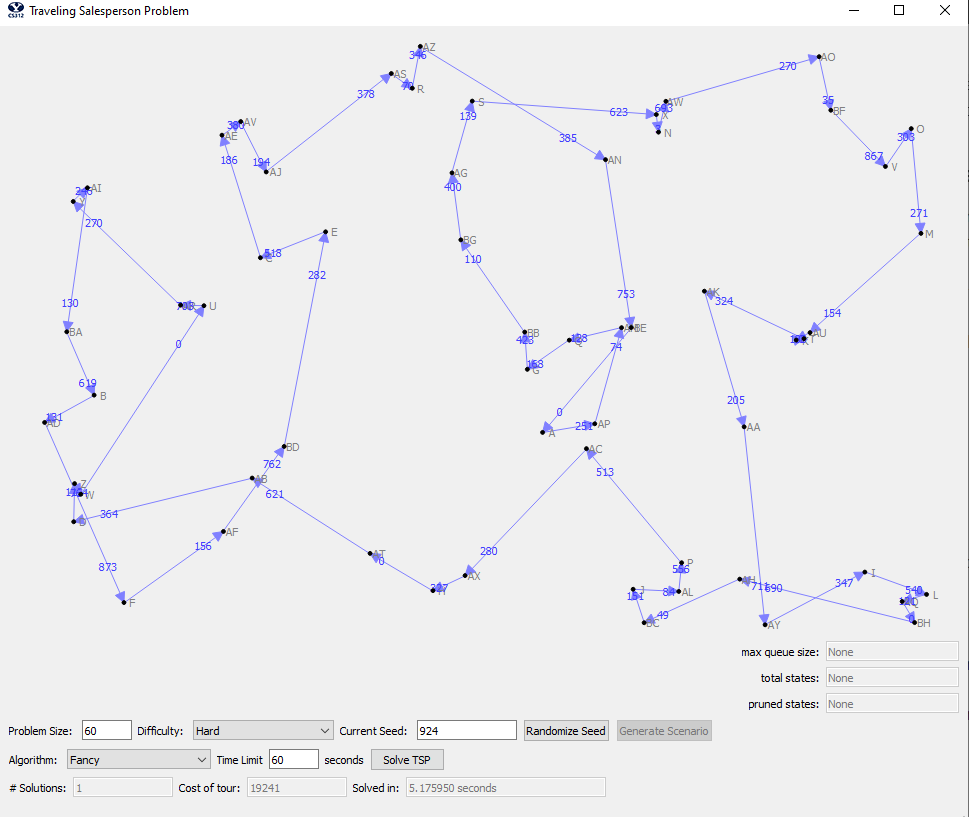
\includegraphics[width=0.35\paperwidth]{sVal100/60_Fancy.png}} \\
        \end{tabular}
    \end{minipage}
\pagebreak

\section{Conclusion}

In conclusion the simulated annealing algorithm proved to carry an increased effectiveness in finding the optimal path of TSP problems over greedy approaches.  The findings listed above showed an 10-13\% reduction in the total cost of a TSP path over a greedy algorithm, and although a greedy approach is favorable in runtime, additional research could greatly increase a simulated annealing’s path finding optimization.  The runtime analysis proved that the difficulty in finding an effective path through simulated annealing is due in part to the randomness inherent to the algorithm itself. Finding valid neighboring paths turns into a guessing game with smaller odds when more cities are involved, but this risk is necessary to escape local minima and expand our search.  This finding shows that a simulated annealing approach would be much more effective at navigating local minima to find a global minimum if our city graph were fully connected and complete.

\pagebreak
\printbibliography

\end{document}